\chapter{Design of the system}
\label{ch:design_of_system}

% OK

Backed by relevant literature and a more philosophical take on how GANs can be deemed creative systems, the design of the system is discussed in this chapter.
The working of the various components is presented loosely based on the CC system description paper by \citet{ventura}.
These components are also placed inside the creative systems framework (CSF) proposed by \citet{csf} to further clarify the creative aspects of the system.

%------------------------------------
\section{Overview of the system}
\label{sec:overview_system}

\begin{figure}[H]
    \centering
    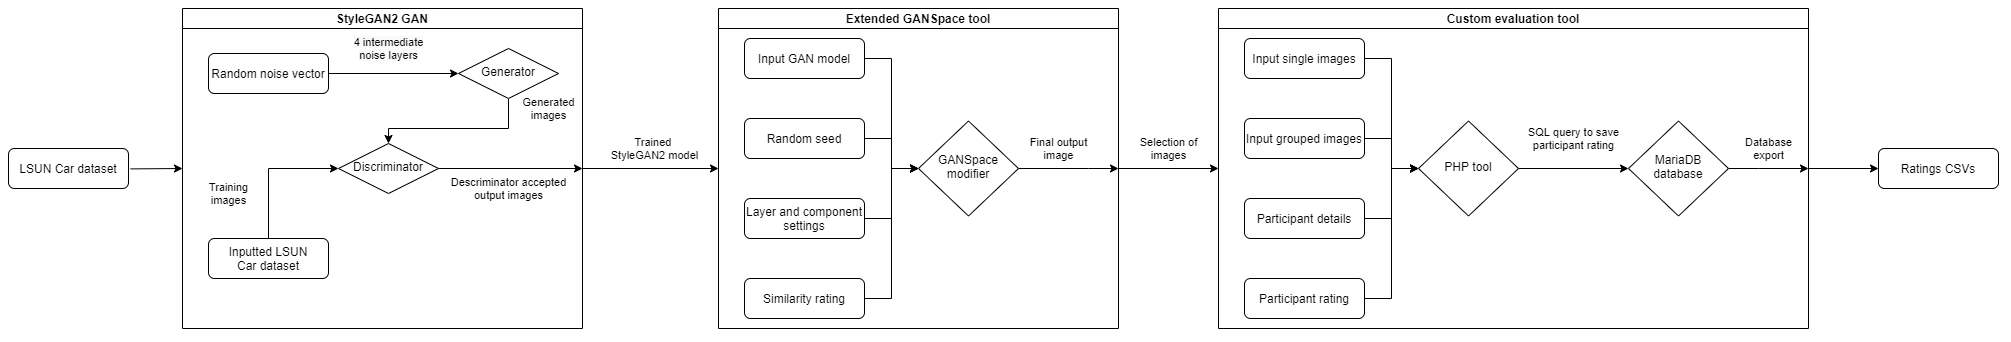
\includegraphics[width=\linewidth]{images/system_overview.png}
    \captionsetup{width=0.7\linewidth}
    \captionsetup{justification=centering}
    \caption{ High level overview of whole creative system's pipeline including external evaluation.  }
    \label{fig:system_pipeline}
\end{figure}

The whole pipeline of the developed system is visualised in figure \ref{fig:system_pipeline}.
For this paper, the first step of training the StyleGAN2 model is bypassed by using a pre-trained one.
The StyleGAN2 car pre-trained model with configuration f is used.
This model generates images of cars at a resolution of 512 by 384 pixels.
It used the LSUN Car dataset for training, which is part of the discussed LSUN-Stanford Car dataset by \citet{cardb}.
It was the highest resolution pre-trained car model at the time of writing.
With the use of an NVIDIA DGX-1 with 8 Tesla V100 GPUs, it took 4 days and 18 hours to train \citep{stylegan2}.
The different components of the extended GANSpace tool, as well as the custom evaluation tool, are discussed later in this paper.

It becomes clear all of the steps and components proposed by \citet{ventura} are in place.
As already discussed, the domain of car design is chosen.
Car design is represented by a phenotypic representation of images of cars.
Internally the genotypic representation of these images is a numerical vector representing the images.
Their exact representation is StyleGAN2 specific.

The used data is the LSUN Car dataset which through conversion to the genotypic representation is used as the knowledge base by the discriminator of the GAN.
The generator function is the generator of the GAN which makes use of four intermediate random noise vectors and more as "input".
More technical details on this can be found in the StyleGAN2 paper \citep{stylegan2}.
Multiple aesthetic measures exist such as the inclusion of required car components, appearance of car brand styling traits and more.
These are mainly taken care of by the discriminator which serves as the value measure.
The similarity rating serves as the novelty measure.
The external evaluation serves as the phenotypic evaluation.

%------------------------------------
\section{Defending the design decisions}
\label{sec:defending_design}

Due to the discussed available resources being rather limited, a pre-trained StyleGAN2 model was the only feasible choice.
The similarity rating is done manually due to limited resources as well, this is further explained later in the paper.
These made design decisions don't limit the creative system of this paper but give rise to interesting future extensions, which are discussed at the end of this paper.

%------------------------------------
\section{Putting it in terms of the CSF}
\label{sec:csf}

A presentation where the system is situated in terms of the CSF was given at the VUB and the used slides are available under the presentations folder of the GitHub repository for this paper \citep{github_project}.
A summary of the contents is given below.
Many different frameworks for describing creative systems exist.
The CSF is chosen as it is formalised the concepts introduced by \citet{boden2004creative} and is created by \citet{csf}, two of the founding figures of CC.
\begin{itemize}
    \item The universe $U$ is Technically all RGB combination of pixels. For the generator, this boils down to all images deemed “real” by the discriminator. When assuming the discriminator does its job, the universe thus consists of all images of realistic-looking cars.
    \item The conceptual space $C$ is the set of all images the generator can make based on all possible noise vectors using its latest transformers. It is clear that $ C \subset U$
    \item Remember from the CSF that $C = [[R]](U)$. This means the rules $R$ constraining the space are the same rules defining the state of the generator.
    \item The rules $T$ are those that introduce randomness and noise as restrictions on the latent spaces. At a high level, the extended GANSpace tool uses these rules to explore the conceptual space.
    \item The rules $E$ are those that define the discriminator as they can be used to assess the quality of the generated image. The similarity rating also belongs to these rules. To keep the language $L$ unchanged, it should be implemented in the same language being a combination of Python and C++.
    \item Since $F^\diamondsuit$ is limited by the output of images having 512 by 384 pixels it is finite. This means $e_c = <R, T, E>^\diamondsuit(\{T\})$ is also finite. Since GANSpace could bypass some of StyleGAN2's rules it is possible that $e_c \not\subset C$.
\end{itemize}